\newpage
\section{TikZ}
与TikZ有关的\LaTeX 中宏包非常丰富,常规的流程图(附录C图\ref{tikzpicture:process}),函数图,电路图等都有对应的宏包支持,
它的语法也不同于Tex。入门TikZ建议看视频,这一块不建议上来就磕文档,官方文档有上千页。当然其绘图功能也是十分强大!

\begin{figure}[h]
    \centering
    % MergeSort-RecursionTree
% Manuel Kirsch
% \documentclass[a4paper,landscape]{scrartcl}
% %%%<
% \usepackage{verbatim}
% \usepackage[active,tightpage]{preview}
% \PreviewEnvironment{tikzpicture}
% \setlength\PreviewBorder{5pt}%
% %%%>

% % \begin{comment}
% % :Title:  Merge sort recursion tree

% % \end{comment}
% \usepackage{fancybox}
% \usepackage{tikz}

% \title{MergeSort-RecursionTree}
% \author{Manuel Kirsch}
% \date{}
% \begin{document}


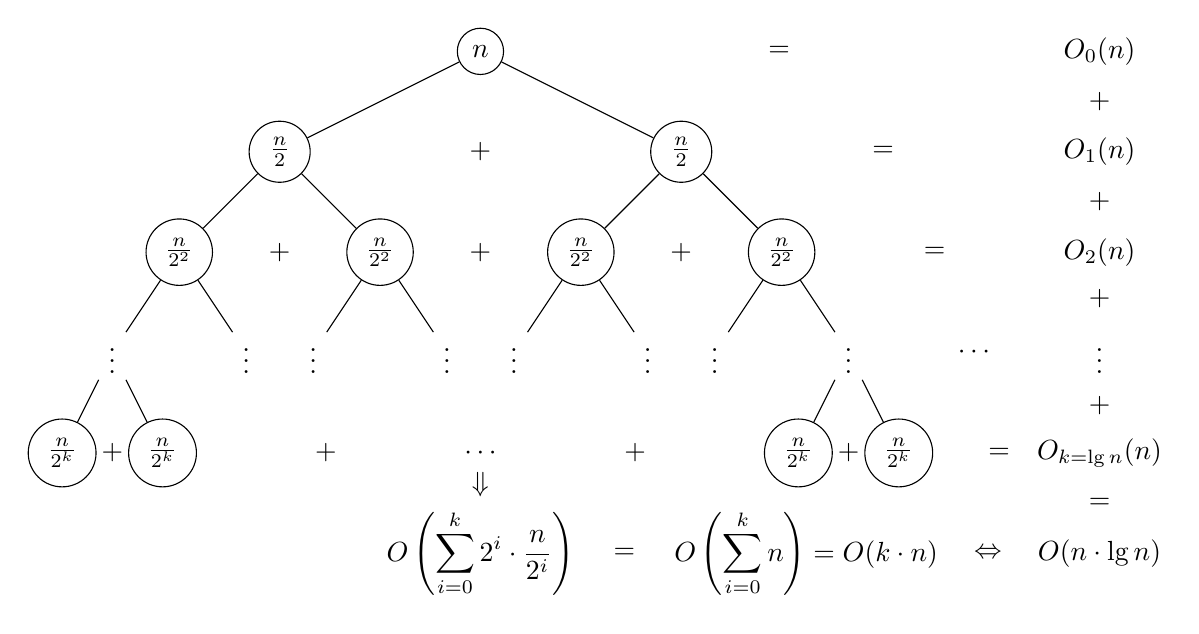
\begin{tikzpicture}[level/.style={sibling distance=60mm/#1},scale=0.85]
\node [circle,draw] (z){$n$}
  child {node [circle,draw] (a) {$\frac{n}{2}$}
    child {node [circle,draw] (b) {$\frac{n}{2^2}$}
      child {node {$\vdots$}
        child {node [circle,draw] (d) {$\frac{n}{2^k}$}}
        child {node [circle,draw] (e) {$\frac{n}{2^k}$}}
      } 
      child {node {$\vdots$}}
    }
    child {node [circle,draw] (g) {$\frac{n}{2^2}$}
      child {node {$\vdots$}}
      child {node {$\vdots$}}
    }
  }
  child {node [circle,draw] (j) {$\frac{n}{2}$}
    child {node [circle,draw] (k) {$\frac{n}{2^2}$}
      child {node {$\vdots$}}
      child {node {$\vdots$}}
    }
  child {node [circle,draw] (l) {$\frac{n}{2^2}$}
    child {node {$\vdots$}}
    child {node (c){$\vdots$}
      child {node [circle,draw] (o) {$\frac{n}{2^k}$}}
      child {node [circle,draw] (p) {$\frac{n}{2^k}$}
        child [grow=right] {node (q) {$=$} edge from parent[draw=none]
          child [grow=right] {node (q) {$O_{k = \lg n}(n)$} edge from parent[draw=none]
            child [grow=up] {node (r) {$\vdots$} edge from parent[draw=none]
              child [grow=up] {node (s) {$O_2(n)$} edge from parent[draw=none]
                child [grow=up] {node (t) {$O_1(n)$} edge from parent[draw=none]
                  child [grow=up] {node (u) {$O_0(n)$} edge from parent[draw=none]}
                }
              }
            }
            child [grow=down] {node (v) {$O(n \cdot \lg n)$}edge from parent[draw=none]}
          }
        }
      }
    }
  }
};
\path (a) -- (j) node [midway] {+};
\path (b) -- (g) node [midway] {+};
\path (k) -- (l) node [midway] {+};
\path (k) -- (g) node [midway] {+};
\path (d) -- (e) node [midway] {+};
\path (o) -- (p) node [midway] {+};
\path (o) -- (e) node (x) [midway] {$\cdots$}
  child [grow=down] {
    node (y) {$O\left(\displaystyle\sum_{i = 0}^k 2^i \cdot \frac{n}{2^i}\right)$}
    edge from parent[draw=none]
  };
\path (q) -- (r) node [midway] {+};
\path (s) -- (r) node [midway] {+};
\path (s) -- (t) node [midway] {+};
\path (s) -- (l) node [midway] {=};
\path (t) -- (u) node [midway] {+};
\path (z) -- (u) node [midway] {=};
\path (j) -- (t) node [midway] {=};
\path (y) -- (x) node [midway] {$\Downarrow$};
\path (v) -- (y)
  node (w) [midway] {$O\left(\displaystyle\sum_{i = 0}^k n\right) = O(k \cdot n)$};
\path (q) -- (v) node [midway] {=};
\path (e) -- (x) node [midway] {+};
\path (o) -- (x) node [midway] {+};
\path (y) -- (w) node [midway] {$=$};
\path (v) -- (w) node [midway] {$\Leftrightarrow$};
\path (r) -- (c) node [midway] {$\cdots$};
\end{tikzpicture}
% \end{document}

    \caption{二叉树}
    \label{tikzpic:tree}
\end{figure}
\begin{figure}[h]
    \centering
     % Pie chart with colors
% Author: Henri Menke
% \documentclass[tikz,border=10pt]{standalone}
% %%%<
% \usepackage{verbatim}
% %%%>
% \begin{comment}
% :Title: Pie chart with colors
% :Tags: Foreach;Charts;Pie charts;Mathematical engine
% :Author: Henri Menke
% :Slug: pie-chart-color

% With this pie chart, we can define a list of colors which is used for the
% pieces. A counter cycles through the list for choosing the color, it restarts
% after the list ended.

% The annotation is done using the pin element.

% This example was written by Henri Menke answering a question of Sascha
% on TeXwelt.de: http://texwelt.de/wissen/fragen/4965/
% \end{comment}
% \begin{document}
\def\angle{0}
\def\radius{3}
\def\cyclelist{{"orange","blue","red","green"}}
\newcount\cyclecount \cyclecount=-1
\newcount\ind \ind=-1


\begin{tikzpicture}[nodes = {font=\sffamily}]
  \foreach \percent/\name in {
      46.6/Chrome,
      24.6/Internet Explorer,
      20.4/Firefox,
      5.1/Safari,
      1.3/Opera,
      2.0/Other
    } {
      \ifx\percent\empty\else               % If \percent is empty, do nothing
        \global\advance\cyclecount by 1     % Advance cyclecount
        \global\advance\ind by 1            % Advance list index
        \ifnum3<\cyclecount                 % If cyclecount is larger than list
          \global\cyclecount=0              %   reset cyclecount and
          \global\ind=0                     %   reset list index
        \fi
        \pgfmathparse{\cyclelist[\the\ind]} % Get color from cycle list
        \edef\color{\pgfmathresult}         %   and store as \color
        % Draw angle and set labels
        \draw[fill={\color!50},draw={\color}] (0,0) -- (\angle:\radius)
          arc (\angle:\angle+\percent*3.6:\radius) -- cycle;
        \node at (\angle+0.5*\percent*3.6:0.7*\radius) {\percent\,\%};
        \node[pin=\angle+0.5*\percent*3.6:\name]
          at (\angle+0.5*\percent*3.6:\radius) {};
        \pgfmathparse{\angle+\percent*3.6}  % Advance angle
        \xdef\angle{\pgfmathresult}         %   and store in \angle
      \fi
    };
\end{tikzpicture}
    

    \caption{扇形图}
    \label{tikzpic:pie}
\end{figure}
\newpage
\begin{figure}[t]
     \centering
     \usetikzlibrary{arrows,shapes,calc,positioning}
\begin{circuitikz}[american]
\draw (0,0) node [scale=1.5,transformer core
] (T){}
      (T.A1) node[above] {A1}
      (T.A2) node[below] {A2}
      (T.B1) node[above left] {B1}
      (T.B2) node[below left] {B2}
      (T.base) node{};
\path (T.B1) -| ++ (2,1) coordinate (tb1){};% define a coordinate at top right relative to B1
\draw (T.B1) -- ++ (0,1) to[D*,-*]  (tb1);
\draw (T.B2) to[D*] ++(2,0)coordinate(tba){} -| (tba |- tb1);
\path (T.B2) |- ++(3,-1) coordinate(tb2){}; % define a coordinate at bottom right relative to B2
\draw (tb2) to[D*,*-] ++(-3,0) -- (T.B2);
\draw (tb2) --(tb2 |- T.B1) to[D*] (T.B1);
% place voltage labels
\draw(T.A1) to[open,v<={$240V_{rms}$,o-o}](T.A2);
\draw($(T.B1)!0.3!(T.B2)$) node[]{$12V_{rms,AC}$}(T.B1);
\draw ($(T.B1)!0.8!(T.B2)$)node[]{$12V_{rms,AC}$}(T.B2);
\draw[thick] ($(T.B1)!0.51!(T.B2)-(1cm,0)$)coordinate[](c){} -- ++ (12.44,0) -| ++ (1,-1) node[ground]{};                          % add a gorund to neutral line
% place capacitors and resistor (upper branches)
\draw(6,1) node[](d1){} to [C,l_=$C_1$, *-*] (c -| d1);
\draw(10,1)node[](d2){} to [C,l_=$C_3$, *-*] (c -| d2);
\draw(13,1)node[](d3){} to [R,l=$R_L$]       (c -| d3);
% place rectangles
\draw (7.5,0.5)  rectangle (8.5,1.5) node[below left= 0.25cm and 0.1cm]{780s};
\draw (7.5,-3.6) rectangle (8.5,-4.6)node[above left=0.25cm and 0.1cm]{790s};
% place capacitors and resistors (lower branches)
\draw(6,-4.15) node[](d4){} to [C,l_=$C_2$, *-*] (c -| d4);
\draw(10,-4.15)node[](d5){} to [C,l_=$C_4$, *-*] (c -| d5);
\draw(13,-4.15)node[](d6){} to [R,l=$R_L$]       (c -| d6);
\draw (8,0.5)  node[](d7){} to [short,-*]        (c -| d7) --(8,-3.6);
% place top and bottom lines
\draw(2,1) -- (7.5,1) (8.5,1) --(11,1) to[short,i^={$I_L$}] (13,1);
\draw(2,-4.15) -- (7.5,-4.15) (8.5,-4.15) --(13,-4.15);
\end{circuitikz}

    \caption{电路图}
    \label{tikzpic:circuit}
\end{figure}

上面的图形都是TikZ代码绘制的,TikZ功能远不止此,由于国内视频缺乏
完整教程,所以学习起来会有些吃力,作者也只是触碰到它的冰山一角,
图\ref{tikzpic:tree} 和图\ref{tikzpic:pie}来自
\url{https://texample.net/tikz},图\ref{tikzpic:circuit}转
载自\href{https://www.latexstudio.net/index/details/index/mid/2302}{latexstudio}。